\documentclass[../main.tex]{subfiles}
\graphicspath{{\subfix{../../Images}}}

\begin{document}
\section{Background}
\label{sec:background}
The following section provides general definitions to the  main concepts that this proposal is built upon. Blockchain technology is still recent but it has matured enough and is sufficiently popular currently to a point that detailed information about it inner workings is actually quite abundant. This section intends to provide sufficient background knowledge for a reader that is not familiar with blockchain technology and related applications.

\subsection{Blockchain}
A blockchain is, essentially, a distributed database. A blockchain is a common data structure to a set of active nodes that compose a \textit{peer-to-peer (P2P) network}. Each of these active nodes has a copy of the common image of the blockchain in their internal storage. The common blockchain image refers to the data structure in which all active nodes of the P2P network agree on. Modification to this image, from here on referred to simply as blockchain, cannot be done outside of the protocol that regulate network operations and a node can only participate in that P2P network if it follows every rule established by the blockchain protocol. Protocol violators are punished, often by mechanisms baked into the protocol itself, and often removed from the network itself.
\par
This allows blockchain to have a somewhat paradoxical nature: digital data uniqueness accomplished through data replication. The security and guarantees of uniqueness in blockchain data are proportional to the size of the network. The more active machines exist replicating \textbf{the same data structure}, the safer the data is because the higher number of potential subversions an adversary is required to do to modify blockchain data outside of the protocol.
\par
Blockchains are append-only databases. This means that the only way to change the blockchain is to add new data to the existing common image. Deletions and modifications are nor allowed by the protocol. As a consequence, blockchains provide levels of transaction transparency that no other tool of that kind ever did: every transaction gets recorded in the blockchain in perpetuity and it is quite trivial to retrieve the historic of operations that affect a given piece of data.
\par
Users interact with blockchains through transactions and transactions themselves are only executed if they display the correct digital signature of the "owner" of the data that can be affected by it. A simple example is a cryptocurrency transfer. Transferring any amount of cryptocurrency between two blockchain accounts changes the state of the blockchain by changing the current balance of each of the accounts affected. Or more simply, adding the transaction that moves funds from account A to account B to the blockchain is, in itself, a change of the state of the blockchain before anything else. It is important to note that this does not violate the "append-only" nature of blockchains: a blockchain account balance is the result of every transaction that ever affected it. New transactions "pile" on top of old ones but these never get deleted or modified. To allow a cryptocurrency quantity to be transferred, blockchains require only a valid digital signature for the "from" account, since it is the one that is going to get its balance diminished. Blockchain accounts are characterized by a pair of asymmetrical encryption keys, with the private one being used to digitally sign transactions in a similar fashion as with regular documents: the digital signature is the transaction text encrypted with the user's private key.
\par
Data is appended to a blockchain with blocks and each block is a collection of transactions. A transaction is considered executed/validated once a block containing it is added to the head of the blockchain. Some applications only consider a transaction as valid once a certain number of blocks have been added on top of the block with the transaction to be validated. Consecutive blocks are connected, i.e., the "chain" in blockchain, using cryptographic hashes. Every subsequent block displays an hash digest that is calculated by concatenating the data in the current block with the hash digest of the previous block and applying the hash function to the combination. Fig \ref{fig:blockchain_example} illustrates this mechanic. A blockchain starts with a genesis block, which is the only one that does not contain a reference to a previous one.

\begin{figure}[htp]
    \centering
    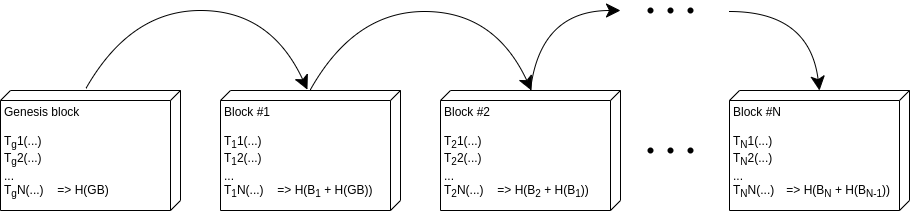
\includegraphics[width=0.9\textwidth]{../Images/01_Blockchain.png}
    \caption{Example of how a generic blockchain is composed of individual blocks cryptographically connected with hash digests.}
    \label{fig:blockchain_example}
\end{figure}

\subsection{Consensus Protocols}
Adding a new block is a critical step of the protocol. Only one active node can do it in each round and different protocols have different strategies to select the node allowed to publish the new block. After that, the remaining nodes update their state of the database with the new block added on top, and that becomes the latest common image until the next round. As an example, Bitcoin uses \textit{Proof-of-Work (PoW)} to select which node gets to add the new block. New blocks are added every 10 minutes and active nodes, also known as miner nodes, try to solve a cryptographic puzzle during that period. This is a computationally intensive operation and the first node to find a solution gets to publish the new block. In most public blockchains that support cryptocurrencies, adding a new block also includes a monetary reward in the form of a newly minted cryptocurrency value. With the popularity of Bitcoin and other PoW based cryptocurrencies, this consensus protocol became progressively problematic due to the high energy cost associated to the enormous amount (and ultimately useless) number of computations required to solve these cryptographic puzzles. In part inspired by this, the blockchain community suggested and adapted more efficient consensus protocols, such as \textit{Proof-of-Stake (PoS)}, where the new block is awarded to a node selected from a group that had previously staked some amount of cryptocurrency. The probability of getting a block is proportional to the amount of cryptocurrency locked in a stake account.
\par
Ethereum was created initially as a PoW blockchain but it switched to a PoS consensus protocol in 2022 due to energy efficiency reasons, but also because it is a more secure and scalable protocol than PoW \cite{ethereum2024}. Another popular consensus protocol is \textit{Proof-of-Authority (PoA)}, where nodes stake their reputation in the blockchain as leverage. Honest behaviour is rewarded and vice-versa. Higher reputations result in higher changes of publishing a new block.

\subsection{Smart Contracts}
The concept of smart contract was developed initially by \cite{Szabo1997} but as a reference to the automation of general-purpose legal contracts. In the blockchain context, this term refers to a script of code, witten in the specific programming language supported by the underlying blockchain, and whose execution runs synchronously on multiple nodes of the network \cite{Zou2021}. The aggregate of computational resources of a network can be organized by a blockchain protocol running in each member, effectively creating a \textit{Distributed Virtual Machine} and this is the main computation platform that executes transactions that can trigger smart contract functions to execute. Due to the lack of a central organizing entity, and to prevent malicious code that can damage this machine, smart contract computations require \textit{gas}, a usually small but significant monetary value in the form of a cryptocurrency supported by the blockchain. The gas required by a smart contract execution is paid when the transaction is submitted, which means that every smart contract execution has a finite amount of gas to execute. This prevents malicious actors from running code that could exhaust the available resources of the virtual machine (by running a script with an infinite loop, for example). When the gas allocated to a transactions runs out, the transaction reverts, i.e., the blockchain recovers the state it had before attempting to run the transaction.

\subsection{Non-Fungible Tokens}
\textit{Non-Fungible Tokens (NFTs)} work paradoxically to regular cryptocurrency tokens. Cryptocurrencies tie an address to a single variable representing the amount of that cryptocurrency the controller of that address owns. NFTs invert this relationship in the sense that they connect the token to an address instead. This clever aspect is part of what guarantees their digital uniqueness: an NFT can have one and only one owner at any point in time. NFTs essentially abstract a piece of data stored distributively in a blockchain and associate it to a single account address that represents the owner of that data. Ownership is ensured by the assumption that the private encryption key from which the account address was derived is under the control of the account owner and no one else.
\par
The non-fungible characteristic of this tokens derives from their inability to be interchanged. With fungible tokens, as with in any cryptocurrencies, each token has a predefined value, can be traded by another one with the same denomination without any loss in value, and can be split and combined into and with fractions of other tokens. Non-fungible tokens cannot be split or combined with others, since each NFT is unique, and implies that there's no direct and fixed correspondence between any two or more NFTs. Fungible tokens are like bank notes: each note has a fixed value, can be exchanged with another with the same value or by a combination of others of smaller values that add to it without any loss in value. Non-Fungible Tokens are akin to paintings or trading cards. Each one is unique, indivisible and usually their value is highly affected from speculation. In the public realm, most NFT applications thus far seem to emulate the analogies considered: they either represent a unique object, such as a painting or any other unique object, or they are used in a collectible setting, in which multiple NFTs are published within the context of a collection. Each token retains its uniqueness because, like physical trading cards, each has a unique identifier that differentiates it from others, even if the remaining metadata is identical to all the other tokens in that collection or series.
\par
The NFTs ability to abstract ownership does not limit itself to digital objects. In fact, a curious argument can be made to use digital NFTs to represent physical, real "ownable objects", which includes everything from a car and a house, to less tangible goods such as ownership of land or intellectual property rights.
\par
NFTs are implemented and can be created (minted) in a smart contract. Blockchains that support NFTs also implement a programming language that allows the creation and deployment of smart contracts that can be used to define and mint these tokens. The actual mechanics behind this process differs significantly per blockchain. This fundamental difference from the cryptographic tokens used as currency expands the scope of applications of blockchain considerably.
\par
NFTs achieve \textit{interoperability} through the implementation of standards. In the Ethereum network, these standards comprise of contract interfaces which define a set of requirements, namely parameters and function signatures, that a NFT token must implement. NFTs that conform to these standards indicate it so in the smart contract that governs them and the implementation of these standards guarantees to other uses a minimum of operability that ensure a secure interface with such token. In the Ethereum network, NFTs are governed by two \textit{Ethereum Improvement Proposals (EIP)}, namely \textit{EIP-721} and \textit{EIP-1155}. These proposals are abstracted into the respective \textit{Ethereum Request for Comments (ERC)} standards \textit{ERC-721} \cite{ERC721} and \textit{ERC-1155} \cite{ERC1155}, which in turn are written as smart contract interfaces that, when implemented in another contract, ensure that the any NFTs minted with that contract contain all the internal mappings required to establish ownership relationships, as well as functions required to transfer the token or to determine its internal parameters, for example.

\subsubsection{Ethereum blockchain}
Ethereum is one of the more popular public blockchains today. It was announced in 2013 through the publication of a whitepaper \cite{Buterin2014}, followed by an \textit{Initial Coin Offering (ICO)} in 2014, and culminating with the official launch of the new blockchain during 2015, through the release of \textit{Frontier}, a early, bare-bone but functional version of the project. Ethereum was launched as a \textit{Proof-of-Work} blockchain, similarly to the only existing public blockchain at that time, Bitcoin, and implemented \textit{Ether (ETH)} as the cryptocurrency of the blockchain. The innovation of Ethereum was its smart contract support, which created a whole new logical and programmable layer on top of it. The community reacted very positively and soon after the first Ethereum smart contract projects begun being deployed in it. ETH is used to pay the \textit{gas} required for their executions, as well as rewarding with newly minted ETH tokens the miner node that solved the cryptographic puzzle for a given round. But like with any other cryptocurrencies with fiat value, ETH can be used as a "normal" currency. By 2022, Ethereum, still in its version 1.0, had grew considerably, and the drawbacks of using a PoW consensus protocol is such large network were becoming quite apparent and prejudicial. As such, this network switched to a PoS consensus protocol during its upgrade to version 2.0.
\par
Ethereum was the first public blockchain to offer smart contract support though its \textit{Ethereum Virtual Machine (EVM)}, and it was also the blockchain where the first NFTs projects were deployed. Ethereum uses Solidity to write smart contracts which in turn are used to define the rules that implement a NFT. In Ethereum NFTs are essentially defined as a combination of synchronised records kept by the implementing contract and that establish a unique relationship between a NFT, identified uniquely by id value, traditionally named \textit{tokenId} in Solidity smart contracts (but not mandatory), and an account address that owns that token. NFT ownership is thus defined as the ability of a user to produce a correctly digitally signed transaction that can change the state of the Ethereum blockchain. This change is mostly restricted to transferring that NFT to a different address, which changes the internal mappings that establish the chain of NFT ownership, therefore triggering the blockchain to change its state. Early NFT projects limit NFT operations to only transfers, but more recent projects take advantage of \textit{dynamic or mutable NFTs}, which are NFTs that allow the owner to change their metadata by exposing functions that allow it \cite{Guidi2023}. For an Ethereum NFT, all records that establish its ownership are centralised in the minting smart contract. Though the actual data is replicated through a series of active nodes, conceptually, all the relationships used for ownership purposes are stored in contract itself as mappings, i.e, key-value structures (known also as \textit{dictionaries} in other programming languages). This means that there is a central point of failure in the Ethereum architecture. If the owner of the contract, or an adversary for that matter, is able to delete the contract, the ownership information is lost irreparably. This type of conceptual centralisation, allied with a fairly high block rate (15 seconds per block in average), make Ethereum difficult to scale, a fact that became evident with the sudden surge in popularity of the \textit{CryptoKitties} project in 2017 \cite{bbc2017}.

\subsubsection{Flow blockchain}
\label{sec:flow_background}
The Flow blockchain was formally launched in October 2020 through the usual \textit{Initial Coin Offering (ICO)} that helped launch most public blockchains in recent years. Flow followed a trend that was addressing the high energy consumption associated to earlier, PoW based blockchains, and established itself with the more efficient and energy friendly PoS consensus mechanism \cite{Hentschel2019a}.
\par
In a PoS based blockchain, new blocks are "mined" by active nodes based on their \textit{stake} on the network, namely, the volume of the blockchain's native cryptocurrency the node currently holds in its account. Higher stakes mean higher probability of being awarded a block publication by the protocol that regulates the network, with the token incentives that such entitles, and vice versa. This process is more energy efficient and faster than the "classical" PoW consensus, where nodes pointlessly spend computer cycles solving cryptographic puzzles only to win a race towards its completion. Given the significant energy waste due to the popularity of PoW blockchains, such as Bitcoin, a blockchain that stays clear of such nefarious protocol is not just a smart choice but a conscientious one as well \cite{Hentschel2019b}.
% // Move this bit to the a more general approach
\par
Flow was created by the same team that created the \textit{CryptoKitties} project in Ethereum, one of the first NFTs based blockchain games in this network to adopt the ERC721 standard for Non-Fungible Tokens. Even though Ethereum was the first one to offer NFT support, it did so on top of a chain that did not envision such applications at the time of its conception. This was evident by the lack of flexibility, inherent security flaws in the code implementing the tokens and its mechanics, as well as a general complexity in writing code and operating with these constructs in the Ethereum network. Ethereum was so ill prepared to deal with the popularity of this initiative that its network went down briefly due to its inability to cope with the added network traffic \cite{bbc2017}. Flow was developed with NFTs support as its main feature, prioritizing NFT creation and mechanics over other applications, a clear contrast over blockchains focused in cryptocurrency transactions \cite{Gharegozlou2019}.

\paragraph{Cadence and the Resource Oriented Paradigm}
\label{sec:cadence_resource_oriented_paradigm}
Flow establishes a new computational paradigm in this context, namely a \textit{Resource Oriented Paradigm (ROP)}. It does so through textit{Cadence}, a smart contract programming language developed for Flow and uses syntax and rules heavily inspired in popular general purpose programming languages such as \textit{Swift, Kotlin, TypeScript}, and \textit{Rust} \cite{Cadence2023}. Cadence establishes ROP through a special type of object, named \textit{Resource}, inspired by the \textit{linear types} popularised by Rust. From a technological point of view, a Resource is akin to a structure or an object from an Object-Oriented context, offering a significant degree of freedom on the type of data that it can encode. But Cadence regulates operations through the notion that every Resource is unique in Flow. This means that Resources need to be accounted at all times, and they cannot be copied, only moved. They can be stored in decentralized storage accounts and loaded from them but, at all times, the Resource is either in storage or out of storage, never in the same state at the same time. These Resources can be created only through smart contracts functions and are exclusive to the Flow blockchain, i.e., not interchangeable with other NFTs from other blockchains.

\par

\begin{figure}[htp]
    \centering
    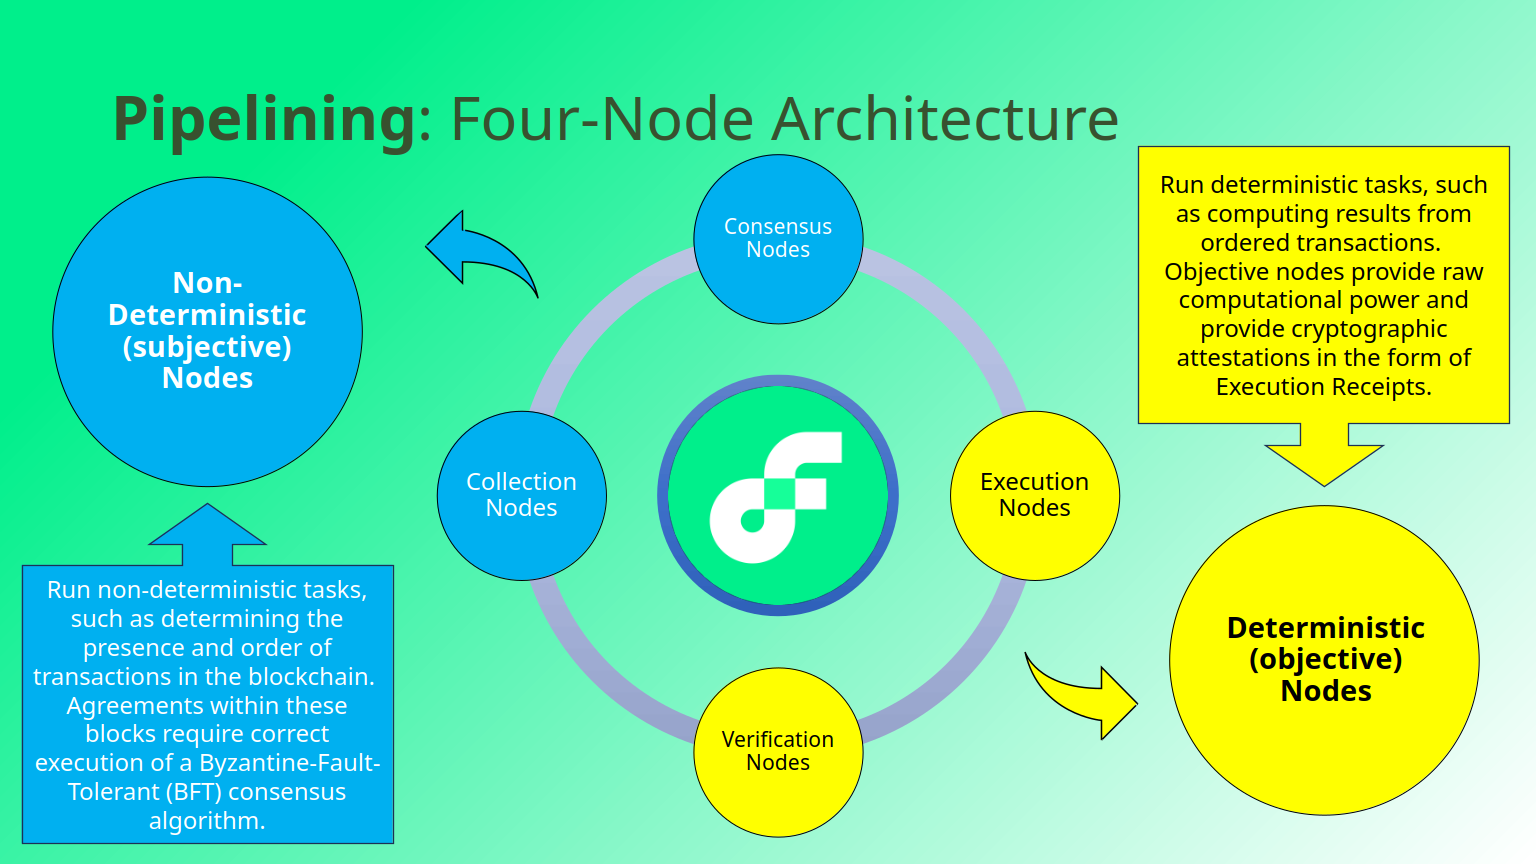
\includegraphics[width=0.9\textwidth]{../Images/03_Flow_architecture.png}
    \caption{The four-node type architecture of Flow \cite{Hentschel2019c}}
    \label{fig:flow_architecture}
\end{figure}

Flow implements a four-node type architecture that implements pipelining to achieve gains in speed, throughput and scalability while keeping minimal costs at a minimum sacrifice in network redundancy. Active nodes in Flow are divided into \textit{Consensus, Collection, Execution} and \textit{Verification} nodes that are organise in a pipeline to optimise computations. Fig. \ref{fig:flow_architecture} provides an overview of the architecture of Flow.

\begin{itemize}
    \item{Consensus Nodes} Decide the presence and order of transactions on the blockchain.
    \item {Collection Nodes} Enhance network connectivity and data availability for applications.
    \item {Execution Nodes} Perform the computation associated with each transaction.
    \item {Verification Nodes} Responsible for keeping the Execution nodes in check.
\end{itemize}

% // NOTE: PoS blockchains don't have miner nodes.
To validate computations, the development team behind Flow developed \textit{Specialised Proofs of Confidential Knowledge (SPoCK)}, a type of non-interactive zero-knowledge proofs based on the \textit{Boneh-Lynn-Shacham (BLS)} signature scheme. These proofs address the \textit{Verifier's Dilemma}, a situation where rational miners are well incentivised to accept unvalidated blocks. Miner nodes in Flow get their block reward by providing a SPoCK that can only be obtained by correctly executing all the transactions that were assigned to it \cite{Ben2020}.
% // TODO: Replace "miner" for validator.


\subsubsection{Storage in Ethereum vs. Flow}
\label{sec:storage_in_flow}
One of the most interesting features that distinguishes Flow from other blockchains, like Ethereum, is its account-based storage model, as opposed to the contract-based one used in Ethereum, for example. In Flow, each user account has its own storage space in the blockchain. Data stored in that space is protected by the same mechanics that prevent someone from transferring a NFT that he/she does not own, transferring cryptocurrencies from another account into his/her own etc. By default only the account controller can access and operate over its storage space. This type of storage decentralisation makes Flow more robust and potentially more scalable, since NFT transactions occur between user accounts and do not have a centralising element that needs to be changed with each transaction that affects a NFT.
\par
Flow employs an \textit{Account-Centric Storage Model} in which storage is the blockchain is based in an account address and the available storage space is proportional to the balance of FLOW token in that account. Due to this, Flow requires a minimum of 0.001 FLOW (around 0.0005\$ at the time of this writing) in the account balance. If an account balance drops bellow this value, the account becomes limited to receive deposits and delete data until the minimum value is restored. Currently, 1 FLOW (~ 0.5\$) allows for 100 MB of on chain storage.
\par
Since Flow saves digital objects in a private storage space associated to an account address, it uses a similar mechanic to how every operating system saves files in local storage: using file paths. Each account storage space is identified by the account address and split into three base domains:
\begin{itemize}
    \item {\textit{Storage}} This is the main private area of storage and only the account owner has any control over it, for both read and write purposes. Resources and other digital object are saved in this domain by default.
    \item {\textit{Public}} The public domain is used to allow controlled read-only access to resources and other digital objects stored in the \verb|\storage| domain.
    \item {\textit{Private}} The private domain is limited to the account owners as well but it works similarly to the \verb|\public| one in the sense it only stores capabilities and not the digital objects themselves. This domain is restricted to only the account owner, unlike the \verb|\public| domain which can be accessed by anyone.
\end{itemize}

Digital objects stored in an account storage space are identified by a storage path obtained by the concatenation of the storage domain and an identifier. For example, an "ExampleNFT" resource saved in the user's storage domain is identified by \verb|\storage\ExampleNFT|. Users have a control to define the identifier to be used in the storage path, as long as it is unique within the domain. This means that, in this example, any other resources saved in the same domain cannot use the "ExampleNFT" identifier anymore.

\begin{figure}[htp]
    \centering
    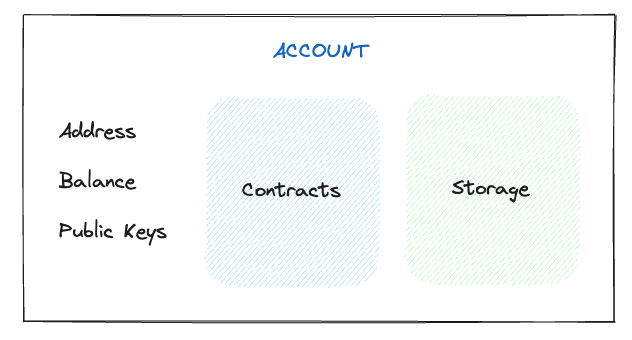
\includegraphics[width=0.85\textwidth]{../Images/08_Flow_Account_Storage_Arch.png}
    \caption{Logical organisation of a Flow account \cite{Cadence2024}}
    \label{fig:flow_account}
\end{figure}

Fig. \ref{fig:flow_account} displays the logical organisation of a user account in Flow. In simple terms, a Flow account is, in itself, a digital object of sorts, defined uniquely by an \textit{address} and a set of \textit{public keys} that are used to validate digital signatures issued by this account. The number of FLOW tokens in the account are available through its \textit{balance} parameter. The account also has a storage area with a size proportional to the \textit{balance} value and it is split into a \textit{contracts} and a general \textit{storage} area. Smart contracts deployed by this account are saved in the \textit{contracts} area, which is publicly accessible so that anyone can verify their code and interact with them, but other digital objects, such as resources, are saved in the private \textit{storage} are. Digital objects stored in this area are private by default, i.e., only accessible to the account owner, but can made public, either as a whole, or limited to certain parameters and functions, by creating and publishing \textit{capabilities} on those resources. Sec. \ref{sec:capabilities} goes into detail about this functionality used to fine tune access control in Flow.

\paragraph{Capabilities}
\label{sec:capabilities}
The \verb|\public| and \verb|\private| domains do not store any objects per se, they store \textit{capabilities} instead. Capabilities are special constructs in Cadence used to delegate access to owned digital objects, i.e., stored in the user's account storage. Users other that object's owner can retrieve a \textit{reference} to an object in someone storage from the corresponding \verb|\public| domain, if the required capability was previously published by the object's owner. Cadence references are very similar to how memory pointers work in other general purpose languages, such as C and C++, but without allowing write access. External users use the references obtained from the \verb|\public| domain to read parameter from the resource, as well as executing functions, as long as these do not change the resource in storage.


\subsubsection{Interacting with the Flow blockchain}
Similar to Ethereum, Flow functions can read and write in the blockchain, namely by executing transactions that trigger the blockchain to change its state (by changing a cryptocurrency balance, minting a new NFT, transfer a NFT to another account, etc), and as in Ethereum, functions that change the state of the blockchain need to be digitally signed by an authorized account.
\par
In Flow, read and write operations are executed with different structures with specific names. If a block of code interacts with a deployed smart contract but it does not changes the state of the blockchain, i.e., it is restricted to data reads, this code can be executed with a Cadence \textit{script}. Scripts do not require signature because they do not consume gas to execute.
\par
On the other hand, if at least one instruction in a block modifies the state of the blockchain, than a Cadence \textit{transaction} needs to be used instead. Fundamentally, transactions are scripts that need a digital signature from an authorized account to execute. Because of it, Cadence transactions are the only context in which the transaction composer has access to a critical \textit{AuthAccount} object that allows access to private elements of the account, such as its internal storage, FLOW token balance, etc. the assumption is that the user has read the transaction itself and knows what types of accesses it executes.
\par
Transactions, scripts and smart contracts in Cadence all have the \verb|.cdc| extension, unlike in Ethereum/Solidity which uses other languages, like Python or Javascript, to write scripts to interact with contract abstractions. The files differentiate themselves by how they are structured: contract files have A \textbf{contract} structure after the imports, also similar to Solidity, transactions are defined similarly, but using the \textbf{transaction} keyword and the code to execute in the transaction structure body. Scripts define a single \textbf{main} function after imports, with the code to run in its body.

\subsubsection{Token standards}
\label{sec:token_standards}
Token standards, for both Fungible and Non-Fungible Token, were created to establish interoperability standards so that different projects in the same network can interact among themselves, namely, cryptocurrencies and NFTs can be traded with minimal effort if users "expect" those tokens to have certain properties and functions. This enforcement is accomplished through token standards, which functionally are contract interfaces. These work very similarly to normal programming interfaces from general purpose languages, like Java for example \cite{Oracle2024}, that define internal parameters and function signatures that are "forced" to be implemented if a class declares the implementation of such interface. If an NFT contract implements the ERC-721 token standard, for example, a user interacting with tokens minted by this contract can access the public internal parameter \textit{tokenId} without having to check the actual contract to see if this parameter was implemented or not. The ERC-721 compliance of the NFT contract guarantees this, along with the remaining parameters and functions.

\paragraph{Ethereum Token Standards}
Ethereum was the first blockchain to welcome and popularize both the NFT concept, but cryptocurrencies in general through the definition of standards. Ethereum projects that followed these token standards created a interoperable ecosystem, where token, but fungible and otherwise, could be traded freely among different contracts within the Ethereum network.
\begin{itemize}
    \item{ERC-20 Fungible Token Standard} The ERC-20 standard regulates the fungible tokens architecture and behaviour in the Ethereum blockchain. These tokens are mostly used as cryptocurrencies. Blockchain projects advertise their ERC-20 compliance as a statement of compatibility with other projects in the Ethereum ecosystem. The standard itself consist in a \verb|.sol| contract interface file written in Solidity \cite{ERC20}.

    \item {ERC-721 Non-Fungible Token Standard} ERC-721 establishes a similar set of rule for smart contracts implementing NFTs. Implementing this interface in a contract forces it to inherit a series of key-value mappings that are used internally to implement the NFT itself, both in terms of ownership record and token metadata \cite{ERC721}.

    \item{ERC-1155 Multi Token Standard} The non-fungible standard in Ethereum was later amended with the ERC-1155 standard to extend the ecosystem to include "semi-fungible tokens". Regular, ERC-721 tokens associate one id to one token. ERC-1155 allows for an id to be associated to a finite set of tokens. Each token with the same id is, effectively, fungible within the same set, a behaviour emulating trading card game, for example.
\end{itemize}

\paragraph{Flow Token Standards}
\label{sec:flow_token_standards}
Flow was created with a different architecture from Ethereum and Cadence is quite different than Solidity, though both achieve similar results. But the similarities in operation with the Ethereum blockchain require that Flow established a similar set of standard for its tokens.

\begin{itemize}
    \item {Fungible Token Standard} Flow's version of the ERC-20 standard is simply named \textit{Fungible Token Standard} \cite{Dapper2022a}, since it was created with the express purpose of regulating fungible tokens in the network, and not as a result for a \textit{request for comments} action. It operates very similarly to the ERC-20 counterpart: the standard itself is an inheritable contract interface in the form of a \verb|.cdc| file \cite{Dapper2022c}, the extension used by the Cadence language, defining a set of parameters and functions that require implementation.

    \item {Non-Fungible Token Standard} For NFTs, Flow implements a single standard, named simply \textit{Non-Fungible Token} \cite{Dapper2022b}, but it does encompass both functionalities from the ERC-721 and ERC-1155 Ethereum standards. It is, in itself, a \verb|.cdc| \cite{Dapper2022d} contract interface file that is imported from implementing contracts. NFTs have a different behaviour in Flow, mainly because of the storage architecture implemented by this blockchain. Flow NFTs are digital object stored in a specific storage path while Ethereum NFTs are, essentially, a series of synchronized key-value mappings that establish a unique relation between an address an token id. Because of this storage difference, Flow NFTs are usually stored inside collections, which are a different, non-unique, type of resource that has the capacity of "holding" multiple NFTs from the same type, i.e., minted from the same contract. This is used primarily to simplify the handling of storage paths, but it essentially mimics the behaviour from the ERC-1155 without an additional standard required.

    \item {MetadataViews} This standard it is used to extend the token functionalities regarding the processing of its metadata, as it is somewhat implied by the standard name. This standard is a much more complex and functional version of the ERC721URIStorage. In fact, Ethereum splits its support to NFT metadata processing in several standards (ERC721URIStorage, ERC721Burnable, ERC721Metadata, ERC721Consecutive, etc.) which need to be imported to expand the support of the contract regarding token metadata processing. Flow simplifies this with one, albeit significantly more complex, standard that includes essentially all the functionalities that Ethereum splits into several standards. It is important to reference this standard, since it is going to be imported by the contract in question, but in order to keep the Solidity and Cadence projects as comparable as possible, we only address the fundamental requirements of the standard, with no additional metadata processing functionalities added to keep the two projects at the same relative level. Flow does put more emphasis in metadata manipulation due to how central NFTs are to this blockchain. At the moment of this writing, Flow has many collectible projects live in its mainnet which do extensive use of this standard to provide tokens that are rich in metadata features. But this commercial aspect of NFT projects are outside of what is intended with this study and, as such, metadata functionalities were kept to a minimum in the Flow implementation of the NFT contract.
\end{itemize}
\end{document}

% // TODO: Add a table to compare both blockchains.
% // TODO: Move the NFT section from a sub one to its own section 
% // TODO: Move the comparison between blockchains to its own section.